\documentclass[pdf,10pt]{beamer}
\mode<presentation>{\usetheme{AnnArbor}}
\usepackage[utf8]{vietnam}
\usepackage{tcolorbox}
\title{\textbf{MA TRẬN - ĐỊNH THỨC}}
\subtitle{Đại số tuyến tính}
\author{\textbf{NHÓM 3}}
\institute{\textcolor{red}{\textbf{Đại học Bách Khoa Hà Nội}}}
\date{Tháng 2, 2022}
\begin{document}

\AtBeginSection[] {
	\begin{frame}{Nội dung}
		\tableofcontents[currentsection, currentsubsection]
	\end{frame}
}

\begin{frame}
	\titlepage
\end{frame}

\section{1. Định nghĩa ma trận}
\begin{frame}{Định nghĩa ma trận}
	Cho $K$ là trường số thực hoặc trường số phức.
	\begin{itemize}
		\item Một ma trận (trên $K$) cỡ $m\times n$ là một bảng có $m$ hàng và $n$ cột:
		    \begin{displaymath}
			A =
			\left (
			\begin{array}{cccc}
				a_{11} & a_{12} & \cdots & a_{1n} \\
				a_{21} & a_{22} & \cdots & a_{2n} \\
				\vdots & \vdots & \ddots &\vdots \\
				a_{m1} & a_{m2} & \cdots & a_{mn} \\
			\end{array}
			\right )
			\end{displaymath}
		với $a_{ij}$ ($\forall i=1,...,m;j=1,...,n$) thuộc trường $K$.
		\item Nếu $m=n$ thì $A$ được gọi là ma trận vuông cấp $n$. Các phần tử $a_{11},a_{22},...,a_{nn}$ được gọi là phần tử chéo. Chúng lập nên \emph{đường chéo chính} của ma trận $A$.
		\item Ký hiệu ma trận có thể dùng dấu ngoặc vuông như trên, hoặc tròn, và thường được ký hiệu gọn là $A= [a_{ij}]_{m\times n}$ hoặc $A= (a_{ij})_{m\times n}$.
	\end{itemize}
\end{frame}

\begin{frame}{Một số loại ma trận}
	\begin{itemize}
		\item Ma trận cỡ $1\times n$ được gọi là ma trận hàng.
		\item Ma trận cỡ $m\times 1$ được gọi là ma trận cột.
		\item Ma trận $A= [a_{ij}]_{m\times n}$ mà mọi phần tử $a_{ij}=0 (\forall i,j)$ được gọi là ma trận không, thường ký hiệu là $\mathcal{O}$, hoặc $\mathcal{O}_{m\times n}$.
		\begin{displaymath}
			\mathcal{O} = 
			\left (
			\begin{array}{cccc}
				0  & 0 & \cdots & 0  \\
				0  & 0 & \cdots & 0  \\
				\vdots & \vdots & \ddots &\vdots \\
				0  & 0 & \cdots & 0  \\
			\end{array}
			\right )
		\end{displaymath}
	\end{itemize}
\end{frame}

\begin{frame}{Một số loại ma trận}
	\begin{itemize}
		\item Ma trận vuông $A= [a_{ij}]_{n\times n}$ được gọi là ma trận tam giác trên nếu $a_{ij}=0$,  với mọi $i>j$.
		\begin{displaymath}
			A =
			\left (
			\begin{array}{cccc}
				a_{11} & a_{12} & \cdots & a_{1n} \\
				0  & a_{22} & \cdots & a_{2n} \\
				\vdots & \vdots & \ddots & \vdots \\
				0 & 0 & \cdots & a_{nn}\\
			\end{array}
			\right )
		\end{displaymath}
		\item Ma trận vuông $A= [a_{ij}]_{n\times n}$ được gọi là ma trận tam giác dưới nếu $a_{ij}=0$, với mọi $i<j$.
		\begin{displaymath}
			A =
			\left (
			\begin{array}{cccc}
				a_{11} & 0 & \cdots & 0 \\
				a_{21} & a_{22} & \cdots & 0 \\
				\vdots & \vdots & \ddots & \vdots \\
				a_{n1} & a_{n2} & \cdots & a_{nn} \\
			\end{array}
			\right )
		\end{displaymath}
	\end{itemize}
\end{frame}

\begin{frame}{Tóm tắt một số loại ma trận}
	\begin{table}
		\centering{
		\begin{tabular}{|l|l|c|}\hline
			\textbf{Tên gọi} & \textbf{Kích cỡ} & \textbf{Ví dụ với $n=3$}\\\hline
			Ma trận hàng (vector hàng) & $1 \times n$ & $\begin{bmatrix}
				3 & 7 & 2
			\end{bmatrix}$\\[1mm]\hline
			Ma trận cột (vector cột) & $n \times 1$ & $\begin{bmatrix}
				4 \\ 1 \\ 8
			\end{bmatrix}$\\\hline
			Ma trận vuông & $n \times n$ & $\begin{bmatrix}
				9 & 13 & 5 \\
				1 & 11 & 7 \\
				2 & 6 & 3
			\end{bmatrix}$\\\hline
		\end{tabular}
		}
		\vspace{2mm}
		\caption{Một số loại ma trận}
		\label{tab:mat-types-1}
	\end{table}
\end{frame}

\begin{frame}{Tóm tắt một số loại ma trận}
	\begin{table}
		\centering{
			\begin{tabular}{|l|l|c|}\hline
				\textbf{Tên gọi} & \textbf{Kích cỡ} & \textbf{Ví dụ với $n=3$}\\\hline
				Ma trận chéo & $n \times n$ & $\begin{bmatrix}
					3 & 0 & 0 \\
					0 & 5 & 0 \\
					0 & 0 & 2 \\
				\end{bmatrix}$\\\hline
				Ma trận tam giác dưới & $n \times n$ & $\begin{bmatrix}
					4 & 0 & 0 \\
					11 & 7 & 0 \\
					5 & 12 & 10
				\end{bmatrix}$\\\hline
				Ma trận tam giác trên & $n \times n$ & $\begin{bmatrix}
					1 & 6 & 4 \\
					0 & 8 & 6 \\
					0 & 0 & 14
				\end{bmatrix}$\\\hline
				
			\end{tabular}
		}
		\vspace{2mm}
		\caption{Một số loại ma trận (tiếp)}
		\label{tab:mat-types-2}
	\end{table}
\end{frame}

\section{2. Các phép toán trên ma trận}
\subsection{2.1. Phép cộng ma trận}
\begin{frame}{Phép cộng ma trận}
	\begin{tcolorbox}
		\textcolor{blue}{Định nghĩa:} Cho hai ma trận cùng cỡ $m \times n$: $A=[a_{ij}]_{m \times n}$, $B=[b_{ij}]_{m \times n}$. Tổng $A + B$ là ma trận cỡ $m \times n$ xác định bởi
		\[
		A+B=[a_{ij}+b_{ij}]_{m \times n}
		\]
	\end{tcolorbox}
	Như vậy muốn cộng hai ma trận cùng cỡ ta cộng các phần tử cùng vị trí.\\[2mm]
	\uncover<2->
	{
	\textit{Ví dụ 1:}\\
	\begin{displaymath}
		\left[
		\begin{array}{cc}
			2 & 3  \\
			-1 & 4 
		\end{array}
		\right] + \left[
		\begin{array}{cc}
			5 & 7 \\
			2 & -3
		\end{array}
		\right] = \left[
		\begin{array}{cc}
			2+5 & 3+7 \\
			-1+2 & 4-3
		\end{array}
		\right] = \left[
		\begin{array}{cc}
			7 & 10 \\
			1 & 1
		\end{array}
		\right]
	\end{displaymath}
	}\\
	\uncover<3->
	{
	\textit{Ví dụ 2:}\\
	\begin{center}
	\begin{math}
		\left[
		\begin{array}{cc}
			1 & 2 \\
			3 & 4
		\end{array}
		\right] + \left[
		\begin{array}{c}
			1 \\ 2 \\ 3
		\end{array}
		\right]
	\end{math}
	\only<4->{không thực hiện được vì hai ma trận \alert<5->{không cùng cỡ.}}
	\end{center}
	}
\end{frame}

\begin{frame}{Các tính chất}
	Cho ma trận $A=[a_{ij}]_{m \times n}$, ta định nghĩa \emph{ma trận đối} của $A$, ký hiệu $-A$ bởi $-A=[-a_{ij}]_{m \times n}$.\\
	Ta cũng định nghĩa $A-B=A+(-B)$.
	
	\uncover<2->{\begin{tcolorbox}
		\textcolor{blue}{Tính chất của phép cộng}\\
		Trên tập hợp các ma trận cùng cỡ $m \times n$ (trên $K$), ta có:
		\begin{itemize}
			\item $(A+B)+C=A+(B+C)$
			\item<3-> $A+\mathcal{O}=\mathcal{O}+A=A$
			\item<4-> $A+(-A)=(-A)+A=\mathcal{O}$
			\item<5-> $A+B=B+A$
		\end{itemize}
	\end{tcolorbox}}
	\uncover<6->{Nói cách khác, tập hợp $\mathcal{M}_{m \times n}(K)$ cùng với phép cộng ma trận lập thành một nhóm giao hoán.}
\end{frame}

\subsection{2.2. Phép nhân ma trận}
\subsubsection{2.2.1. Nhân một số với ma trận}
\begin{frame}{Phép nhân một số với ma trận}
	\begin{tcolorbox}
		\textcolor{blue}{Định nghĩa} \\
		Tích của số $k$ với ma trận $A = [a_{ij}]_{m \times n}$ là ma trận $kA$ cỡ $m$ × $n$ cho bởi
		\begin{displaymath}
			kA = [ka_{ij}]_{ m \times n }.
		\end{displaymath}
	\end{tcolorbox}
	
	Khi nhân một số $k$ với ma trận, ta nhân mỗi phần tử của ma trận với $k$.\\[2mm]
	\textbf{Ví dụ:}
		\begin{displaymath}
			2 
			\left[
			\begin{array}{ccc}
				1  & 2 & 3 \\
				4  & 5 & 6 
			\end{array}
			\right]
			=
			\left[
			\begin{array}{ccc}
				2  & 4 & 6 \\
				8  & 10 & 12 
			\end{array}
			\right]
		\end{displaymath}
	\textbf{Chú ý:}
	Ta có $(-1)A = -A$
\end{frame}

\begin{frame}{Tính chất}
	\begin{tcolorbox}
		\textcolor{blue}{Tính chất cơ bản}  \\
		Cho $A,B$ thuộc $\mathcal{M}_{m \times n}(K)$ và $c,d \in K$. Khi đó
		\begin{itemize}
			\item $(cd)A=c(dA)$,
			\pause
			\item $1A=A$,
			\pause
			\item $c(A+B)=cA+cB$,
			\pause
			\item $(c+d)A=cA+dA$.
		\end{itemize}
	\end{tcolorbox}
	\uncover<5->
	{
	Tính chất bổ sung: Cho $A$ là ma trận cỡ $m \times n$, $\mathcal{O}$ là ma trận không cỡ $m \times n$:
	\begin{displaymath}
		cA = \mathcal{O} \Rightarrow
		\left[
		\begin{array}{cll}
			c & = & 0  \\
			A & = & \mathcal{O} 
		\end{array}
		\right.
	\end{displaymath}
	}
\end{frame}

\subsubsection{2.2.2. Nhân hai ma trận}
\begin{frame}{Phép nhân hai ma trận}
	\begin{tcolorbox}
		\textcolor{blue}{Định nghĩa}\\
		Cho hai ma trận $A= [aij]_{m \times n}$ cỡ $m \times n$ và $B = [bij]_{n \times p}$ cỡ $n \times p$. Tích $AB$ là ma trận $C = [cij]_{m \times p}$ cỡ $m \times p$ cho bởi
		\begin{displaymath}
			c_{ij} = a_{i1}b_{1j} + a_{i2}b_{2j} + ... + a_{in}b_{nj} = \sum_{k=1}^{n} a_{ik}b_{kj} (\forall i=1,...,m;j=1,...,p).
		\end{displaymath}
	\end{tcolorbox}
	\begin{figure}[tbh]
		\centering{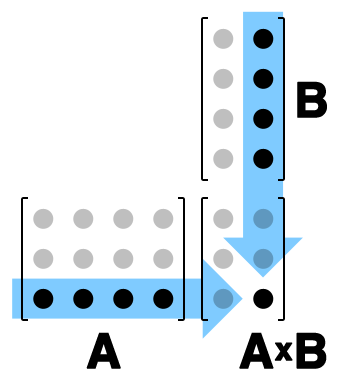
\includegraphics[scale=0.2]{Picture2.png}}
		\caption{Minh họa phép nhân hai ma trận}
		\label{fig:mult}
	\end{figure}
\end{frame}

\begin{frame}{Chú ý}
	\begin{itemize}
		\item Tích $AB$ chỉ được định nghĩa khi số cột của $A$ bằng số hàng của $B$.
		\item Ta có thể tính phần tử $ij$ của ma trận $AB$ bằng cách nhân lần lượt $n$ phần tử của dòng thứ $i$ của $A$ (từ trái sang phải) với $n$ phần tử của cột thứ $j$ của $B$ (từ trên xuống dưới) rồi lấy tổng của chúng: \\
		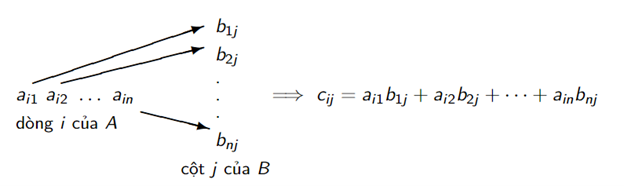
\includegraphics[width=3.7in]{Picture1.png}
		\item Có thể tích $AB$ tồn tại nhưng tích $BA$ không tồn tại. Kể cả trong trường hợp $AB$ và $BA$ đều tồn tại thì nói chung $AB \neq BA$.
	\end{itemize}
\end{frame}

\begin{frame}{Chú ý}
	\begin{itemize}
		\item Nói chung $AB = \mathcal{O}$ không suy ra được $A= \mathcal{O}$ hoặc $B= \mathcal{O}$.
		\item Nói chung $AC = BC$ ( hoặc $CA = CB$ ) với $C \neq \mathcal{O}$ không suy ra được $A = B$
	\end{itemize}
	\begin{flushleft}
		\textbf{Ví dụ:}
	\end{flushleft}
	\begin{itemize}
		\item 
		$A = \left[ 
		\begin{array}{rr}
			1 & 1 \\
			2 & 2 
		\end{array}
		\right]
		$, $B = 
		\left[
		\begin{array}{rr}
			1 & -2 \\
			-1 & 2 
		\end{array}
		\right]$:
		$A \neq \mathcal{O}$, $B \neq \mathcal{O}$ nhưng $AB = \mathcal{O}$,
		
		\item $
		A = \left[ 
		\begin{array}{rr}
			1 & 0 \\
			2 & 0 
		\end{array}
		\right]$, 
		$B = 
		\left[
		\begin{array}{rr}
			0 & -1 \\
			0 & -2 
		\end{array}
		\right]$,
		$C = \left[
		\begin{array}{rr}
			1 & -2 \\
			-1 & 2 
		\end{array}
		\right]$: \\[3mm] $AC = BC = 
		\left[
		\begin{array}{cc}
			1 & -2  \\
			2 & -4 
		\end{array}
		\right]$ nhưng $A \neq B$
		
	\end{itemize}
	
\end{frame}

\begin{frame}{Ví dụ}
	
	Cho $A = \left[ 
	\begin{array}{rrr}
		1 & -1 & 2  \\
		0 & 1 & -2 
	\end{array}
	\right]$, 
	$B = \left[
	\begin{array}{rr}
		1 & 2 \\
		2 & -1 \\
		3 & 1 
	\end{array}
	\right]$.
	Tính $AB$.
	\begin{itemize}
		\item $C = AB$ cỡ $2 \times 2$, $C = \left[ \begin{array}{rr}
			C_{11}  & C_{12} \\
			C_{21} & C_{22} 
		\end{array}
		\right] $.
		\item $C_{11}=1.1+(-1).2+2.3=5 .$
		\item $C_{12}=1.2+(-1).(-1)+2.1=5 .$
		\item $C_{21}=0.1+1.2+(-2).3=-4 .$
		\item $C_{22}=0.2+1.(-1)+(-2).1=-3 .$
		\item $AB=C= \left[ 
		\begin{array}{rr}
			5     &  5 \\
			-4     & -3 
		\end{array}
		\right] $.
	\end{itemize}
\end{frame}

\begin{frame}{Tính chất}
\begin{tcolorbox}
\textcolor{blue}{Tính chất} \\[2mm]
Cho $A,B,C$ là các ma trận với cỡ sao cho các phép toán trong các hệ thức sau được định nghĩa. Cho $c \in K$. Khi đó:
\begin{itemize}
	\item $(AB)C=A(BC)$
	\item $A(B+C)=AB+AC$, $(B+C)A=BA+CA$
	\item $(cA)B=A(cB)=c(AB)$
	\item Cho $A$ cỡ $m \times n$: $AI_{n} = A$ và $I_{m} A = A$.
\end{itemize}
\end{tcolorbox}
\textbf{Nhận xét}: Tập $\mathcal{M}_{n}(K)$ các ma trận vuông cấp $n$ cùng với các phép toán cộng và nhân ma trận lập thành một vành (có đơn vị).
\end{frame}

\subsection{2.3. Lũy thừa ma trận}
\begin{frame}{Lũy thừa ma trận}
	Cho $A$ là ma trận vuông cấp $n$.
	\begin{itemize}
		\item Với $k \ge 1$ là một số nguyên dương, ta định nghĩa
		\begin{displaymath}
			A^{k}=A.A...A
		\end{displaymath}
		\item Tính chất : $A^{k+I} = A^k A^I, A^{KI} = (A^K)^I$, với mọi $K,I$ nguyên dương \\
		\item Với $f(x) = a_k x^k + ... + a_1 x + a_0$ là một đa thức bậc $k$, ta định nghĩa
		\[f(A)=a_k A^k + ... + a_1 A + a_0 I_n\]
	\end{itemize}
\end{frame}

\subsection{2.4. Ma trận chuyển vị}
\begin{frame}{Phép chuyển vị ma trận}
	\begin{block}{Chuyển vị ma trận}
		Cho $A = [a_{ij}]_{m\times n} $ cỡ $m \times n $. Ma trận chuyển vị của $A$, ký hiệu $A^T = [b_{ij}]$ là
		ma trận $m \times n $ xác định bởi
		\begin{displaymath}
			b_{ij} = a_{ij}, \forall i = 1,...n;j=1,...,m.\end{displaymath}
	\end{block}\ \\
	Các cột của $A^T$ là các hàng của $A$. Các hàng của $A^T$ là các cột của $A$.\\[2mm]
	\textit{Ví dụ:}\\
	\centering
	{
	\begin{math}
		A = \left(
		\begin{array}{cc}
			0 & 1 \\
			3 & 2
		\end{array}
		\right )
	\end{math} thì
	\begin{math}
		A ^T = \left(
		\begin{array}{cc}
			0 & 3 \\
			1 & 2
		\end{array}
		\right)
	\end{math}
	}
\end{frame}

\section{3. Định thức ma trận vuông}
\begin{frame}{Định nghĩa định thức}
	Cho $A = [a_{ij}]_{n \times n}$ là một ma trận vuông cấp $n$. Ta sẽ định nghĩa định thức của $A$, ký hiệu $\det(A)$ hoặc $|A|$, truy hồi theo $n$.
	\begin{block}{Định thức ma trận cấp 1 và 2}
		\begin{itemize}
			\item Nếu $A =[a_{11}]$ là ma trận cấp 1, thì $\det(A)=a_{11}$.
			\\[5mm]
			\item Nếu $A = 
			\begin{bmatrix}
				a_{11} & a_{12} \\
				a_{21} & a_{22}
			\end{bmatrix} $
			thì\\[5mm]
		\end{itemize}
		\centerline{
			$\det(A)=
			\begin{vmatrix}
				a_{11} & a_{12} \\
				a_{21} & a_{22}
			\end{vmatrix}
			= a_{11}a_{22} - a_{12}a_{21}.$
		}
	\end{block}
	
\end{frame}

\begin{frame}{Định thức ma trận cấp $n \geq 3$}
	Giả sử ta đã định nghĩa được định thức của tất cả các ma trận vuông cấp $n - 1$.
	\begin{itemize}
		\item Xét ma trận $A = [a_{ij}]_{n \times n}$ là một ma trận vuông cấp $n$.
		\item Với mỗi $i$, $j$, ta gọi $M_{ij}$ là ma trận nhận được từ $A$ bằng cách xóa đi cột $i$ và $j$. Khi đó $M_{ij}$ là một ma trận vuông cấp $n-1$.
		\item Đặt $A_{ij}=(-1)^{i+j}det(M_{ij}$), và $A_{ij}$ được gọi là phần phụ đại số của $a_{ij}$.
	\end{itemize}
	\begin{block}{Định nghĩa}
		Định thức của $A=[a_{ij}]_{n \times n}$ là
		\\[5mm]
		\centerline{ $\det(A)=|A|=a_{11}A_{11}+a_{12}A_{12}+\dots+ a_{1n}A_{1n}.$ }
	\end{block}
\end{frame}

\begin{frame}{Ví dụ}
	\ \\[-3mm]
	Tính định thức của ma trận A =
	$\begin{bmatrix}
		1 &  2 & -1 \\
		2 & -1 &  2 \\
		3 &  1 &  2 
	\end{bmatrix} $
	
	\begin{itemize}
		\item $M_{11}=
		\begin{vmatrix}
			-1 & 2  \\
			1 & 2  
		\end{vmatrix}
		\Rightarrow A_{11} = + \det(M_{11}) =
		\begin{vmatrix}
			-1 & 2  \\
			1 & 2  
		\end{vmatrix}
		= -4 $
		\item $M_{12}=
		\begin{vmatrix}
			2 & 2  \\
			3 & 2  
		\end{vmatrix}
		\Rightarrow A_{12} = - \det(M_{12}) =
		\begin{vmatrix}
			2 & 2  \\
			3 & 2  
		\end{vmatrix}
		=-(-2)=2
		$
		\item $ M_{13}=
		\begin{vmatrix}
			2 & -1  \\
			3 &  1  
		\end{vmatrix}
		\Rightarrow A_{13} = + \det(M_{13}) =
		\begin{vmatrix}
			2 & -1  \\
			3 &  1  
		\end{vmatrix}
		=5 $
		\item
		$
		|A|=a_{11}A_{11}+a_{12}A_{12}+a_{13}A_{13} = 1.(-4)+2.2+(-1).5=-5
		$
	\end{itemize}\ \\[2mm]
	Viết gọn:
	\begin{eqnarray*}
		|A|  & = & a_{11} \det(M_{11})-a_{12} \det(M_{12}) + a_{13} \det(M_{13}) \\
		& = & 
		1.\begin{vmatrix}
			-1 & 2 \\
			1 &  2  
		\end{vmatrix}
		-2.
		\begin{vmatrix}
			2 & 2  \\
			3 & 2  
		\end{vmatrix}
		+(-1).
		\begin{vmatrix}
			2 & -1  \\
			3 &  1  
		\end{vmatrix}\\
		& = & 1.(-4)+2.2+(-1).5 =-5.
	\end{eqnarray*}
\end{frame}

\section*{Tài liệu tham khảo}
\begin{frame}{Tài liệu tham khảo}
	\begin{itemize}
		\item Bài giảng Đại số, \textit{PGS. TS. Nguyễn Duy Tân, tháng 10 - 2021}
		\item Bài giảng Đại số tuyến tính, \textit{TS. Bùi Xuân Diệu, tháng 9 - 2019}
		\item \href{https://vi.wikipedia.org/wiki/Ma_tr\%E1\%BA\%ADn_(to\%C3\%A1n_h\%E1\%BB\%8Dc)}{Ma trận (toán học) - \textit{Wikipedia}}
	\end{itemize}
\end{frame}

\end{document}